% This is samplepaper.tex, a sample chapter demonstrating the
% LLNCS macro package for Springer Computer Science proceedings;
% Version 2.20 of 2017/10/04
%
\documentclass[runningheads]{llncs}
%
\usepackage{graphicx}
\usepackage{amsmath}
% Used for displaying a sample figure. If possible, figure files should
% be included in EPS format.
%
% If you use the hyperref package, please uncomment the following line
% to display URLs in blue roman font according to Springer's eBook style:
% \renewcommand\UrlFont{\color{blue}\rmfamily}
\usepackage[numbers,sort&compress]{natbib}
\begin{document}
%
\title{Learning Spectral Representations:\\ Semantic Memory and the\\ Information Dynamics of Thinking}
%
\titlerunning{Learning Spectral Representations}
% If the paper title is too long for the running head, you can set
% an abbreviated paper title here
%
\author{Steve~Homer\inst{1}\orcidID{0000-1111-2222-3333} \and
Geraint~A.~Wiggins\inst{1,2}\orcidID{0000-0002-1587-112X}}
%
\authorrunning{S.~Homer and G.~A.~Wiggins}
% First names are abbreviated in the running head.
% If there are more than two authors, 'et al.' is used.
%
\institute{AI Lab, Vrije Universiteit Brussel, 1050 Brussels, Belgium \and
School of Electronic Engineering and Computer Science,\\Queen Mary University of London, Mile End Road, London E1 4FZ, UK \\
\email{steven.t.homer@gmail.com,geraint@ai.vub.ac.be}}
%
\maketitle              % typeset the header of the contribution
%
\begin{abstract}
The abstract should briefly summarize the contents of the paper in
150--250 words.

\keywords{Statistical learning  \and Representation Learning \and Information Dynamics.}
\end{abstract}
%
%
%
\section{Introduction}
This paper presents progress in statistical knowledge representation applied to auditory input, specifically speech. The work has been conducted in the context of a longer-term project, on the Information Dynamics of Thinking (IDyOT). Until the current publication, the work has focused either on theoretical explication \cite{Wiggins12,WigginsForth15,ForthAgresEtAl16,vanderVeldeForthEtAl17,Wiggins18}, or on statistical modelling applied to textual data \cite{WigginsSanjekdar19}. In this paper, we begin to explore the potential of the IDyOT theory to learn its own representations and build hierarchical ``deep'' representations of meaning. At this stage, we do not claim that these representations are cognitively valid; rather we attempt just to demonstrate that the proposal is capable of learning from data in the way proposed, and that the representations produced are credible as the output of a human-like learning system. The key contribution of the present paper is the use of spectral approaches to knowledge representation and the extraction of knowledge from time-variant speech information in the context of structural analysis by statistical model.

In the following sections, we first outline the context of the Information Dynamics of Thinking project, and summarise it. We then explain the detail of our implementation. We detail the empirical studies we have conducted to test whether the theory identifies perceptual and semantic categories as predicted. Finally, we discuss the prospects for future work on the model.
\section{Background}
\subsection{Overview}
\begin{figure}[t]
    \centering
    \resizebox{.9\linewidth}{!}{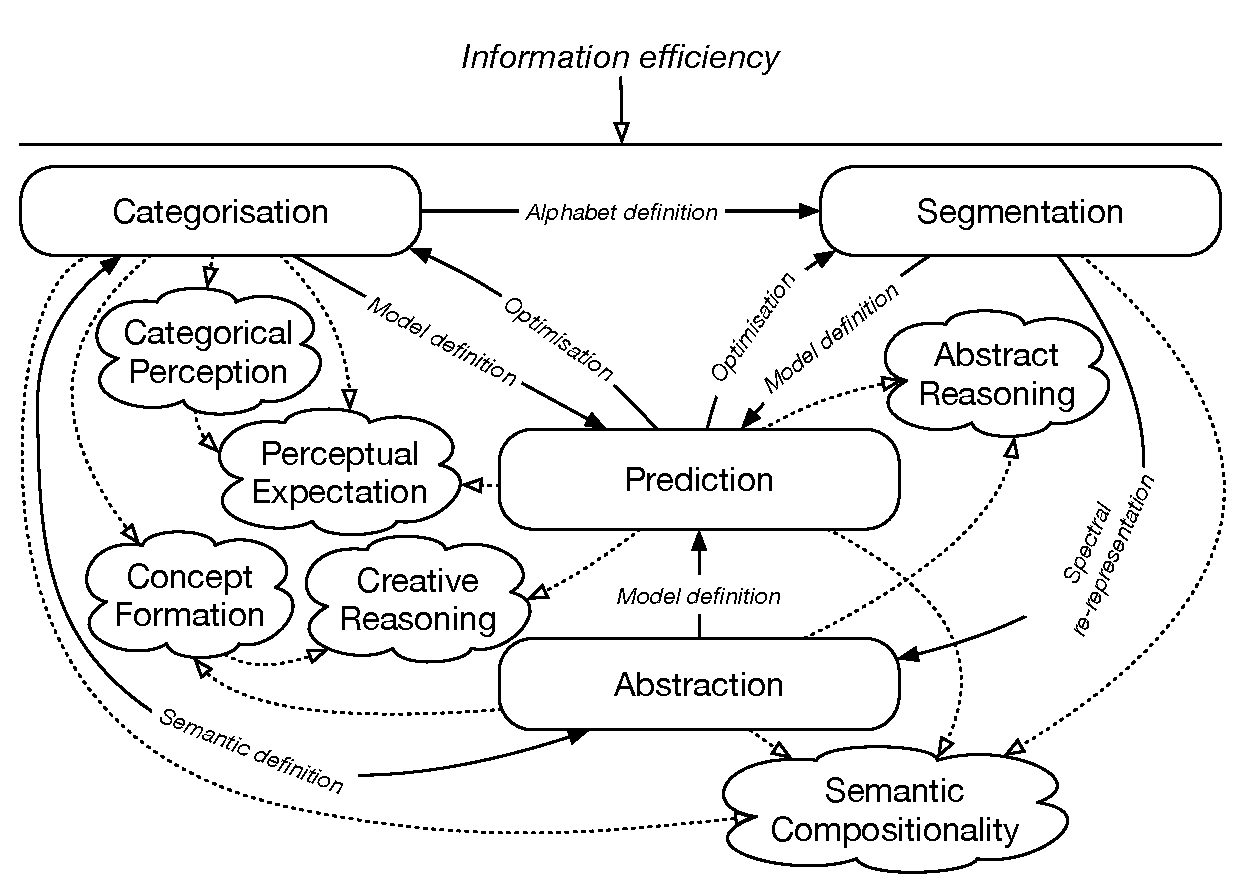
\includegraphics{pix/overview}}
    \caption{Overview of IDyOT components and operation cycle. Rounded boxes are the main IDyOT processes. Cloud shapes represent the phenomena explicated. Arrows are labelled with the operations that connect the main processes. The whole is guided by the information efficiency criterion. Figure and caption reproduced under CC-BY license \cite{WigginsSanjekdar19}.}
    \label{fig:IDyOToverview}
\end{figure}
The theory of Information Dynamics of Thinking (IDyOT) is an attempt to capture in an implemented computational model a hypothetical fundamental cognitive process. That process, it is claimed, drives cognition and action in a mind. The theory draws together the processes of (implicit, non-conscious) learning, segmentation of sequences in time, construction of categorical perceptual and semantic representations, and abstraction of data into ontological hierarchies. The motivation of the theory is to be able to predict what happens next in the world, so it accords mostly with the approach of Clark \cite{Clark13}. Like many such theories, it is based on statistical modelling (viewed as a simulation of cognitive process, not as a model of data) and Shannon information theory \citep{Shannon48}. The theory is formulated as one of ``information dynamics'', and not as one of ``free energy''  \citep{Friston10}, because there is evidence (from music cognition studies  \citep{Huron06,PearceWiggins12,HansenPearce14}) that humans are directly sensitive to the quantity of Shannon entropy in perceived data, and so  grander physical metaphor is superfluous.

The IDyOT process is illustrated in Fig.~\ref{fig:IDyOToverview}. It operates over 
% this bit taken directly from Frontiers paper - needs reworking
input sequences at a given basic level of representation---here, the vectors of a Fourier Transform of human speech. These sequences are segmented using boundary entropy \cite{SproatShihEtAl94}, which we explain below. Each segment so produced is then represented as a temporal trajectory in a geometrical space of dimension and scale appropriate to its particular input type.  This space becomes the semantic space of the data level with which it is associated. As the sequence is so segmented and recorded, a superordinate sequential and semantic layer is constructed, from vectors determined by spectral transforms of the multidimensional sequences at the subordinate layer. The representations are spectral because this mathematical approach allows comparison of sequences of varying lengths, each represented by a single point in the superordinate space; in our case, the spectral transformation is the standard Fourier Transform \cite{?}. In the current initial experiments, the geometry of the superordinate space is Euclidean. However, in general, that geometry is constructed by an inner product function that induces a norm (distance) that models similarity in this particular space.

The whole process is guided by an information efficiency criterion, expressed domain-independently in terms of a Shannon-type estimate of the average number of bits required to represent each symbol in the learned memory. In what follows, we refer to this quantity as {\it mean information content}; the estimated number of bits to required to represent a signal is called the {\it information content}.




\subsection{Perceptual Segmentation by Boundary Entropy}
\subsection{Conceptual Spaces}
\cite{Gardenfors00,Gardenfors14}
\subsection{Spectral Representations of Meaning}
\cite[][\S7.2.5]{Wiggins18}
\subsection{The Information Dynamics of Thinking}

\paragraph{Segmentation}
\paragraph{Categorisation}
\paragraph{Abstraction}
\paragraph{Prediction}

%%%%%%%%%%%%%%%%%%%%%%%%%%%%%%%%%%%%%%%%%%%%%%%%%%%%%%%%%%%%%%%%%%%%%%%%%%%%%%%

\section{Implemented Model}
{\it Steve to do from here on...}

%%%%%%%%%%%%%%%%%%%%%%%%%%%%%%%%%%%%%%%%%%%%%%%%%%%%%%%%%%%%%%%%%%%%%%%%%%%%%%%

\subsection{Abstraction}

\subsubsection{Hilbert Spaces}
In order to represent the spectral transformations of we utilize the mathematical formalism of the Hilbert Space.  Hilbert spaces are complete inner product spaces.  That is, a Hilbert space is a vector space equipped with an inner product, but is also complete -- the space is big enough to include the norm of converging sequences.  In the case of an infinite-dimensional Hilbert space, this completeness criterion cannot be taken for granted, but in the finite-dimensional case, the space is always complete.  Importantly, a Hilbert space has a norm induced by the inner product, which allows us to talk about distances between vectors, something that we require of a formalism of conceptual spaces.

What makes Hilbert spaces powerful is the ability to represent a function as a point in the space.  With the aid of the inner product, one can produce an (infinite) orthonormal sequence for the Hilbert space, and by decomposing the function into its Fourier series on that sequence, we can recover a corresponding coefficient for each element of the orthonormal sequence.  By thinking of each of these elements as a dimensions, we can arrange those coefficients into a vector, thereby representing the function as a point in the Hilbert space.

Hilbert Space Equations

\subsubsection{Fourier Transform Operator}
In the abstraction process, we would like to produce a spectral representation of a segment.  One way of doing this is by taking the Fourier transform to take the representation of a segment from the time-domain to the frequency-domain.  By taking the Fourier transform of a time-varying signal, we produce the frequency-domain coefficients for each orthogonal frequency.  By taking the Fourier transform of a curve in a Hilbert space, we end up with a frequency-domain representation of that curve.

The Fourier transform is an integral operator on Hilbert spaces.  An operator takes an input function and produces an output function, and so when thinking in terms of finite-dimensional Hilbert spaces, an operator will take the input from one domain to another, but does not change the shape of that input.  This has ramifications discussed below.

The abstraction process will then consist of taking the Fourier transform of a trajectory through a Hilbert space, and then viewing the resulting frequency-domain signal as a point in the superordinate space.

\subsubsection{Tensor Rank Promotion}

A segment in the sequential memory corresponds to a trajectory in the semantic memory.  As such, a trajectory is a curve through the points representing those elements of the segment.  For example, if each point is represented as a vector, a sequence of those points would be a vector of vectors, i.e. a matrix.  Since the Fourier transform is an operator, it maintains the shape of the trajectory, and since we will view the result of the Fourier transform as a point in the superordinate space, the result is a space with one higher rank.  Hence, each level of abstraction promotes the rank of the tensors by one.  

To clarify the first few stages of this process, we begin at the base abstraction layer, whose space is filled with points representing the frequencies of a signal of a short moment of time.  These points are vectors (tensor rank 1), that, when strung together into a trajectory, form a matrix.  By taking the Fourier transform and viewing the result as a point in the superordinate abstraction layer, that upper layer is now composed of points represented as matrices (tensor rank 2).  Again, we can string this points together, forming a cube, for a trajectory, take the Fourier transform, and view it as a point in the superordinate layer.  Now this layer is composed of points represented as cubes (tensor rank 3). Repeating this process, we increase the rank of the representative tensor by one for each layer of abstraction.

Unfortunately, this leads to an exponential explosion in the number of elements of constituting a point in a given layer.  Formally, $r^\alpha$, where $r$ is the resolution of interpolation (discussed below), usually a small power of two, and $alpha$ is the level of the abstraction layer.  Though this is not really a problem theoretically, it has consequences in terms of implementation.

Diagram of Tensor Promotion

\subsubsection{Component-wise Independence}

When performing the Fourier transform on a tensor of any rank, it should be noted that each component in the tensor is independent from every other component.  Though this is not necessarily true in general, due to the particular hierarchical construction of these spaces, each component is decoupled from the rest.  Starting at the bottom, the time-domain sound signal is transformed into a frequency-domain signal of coefficients in independent frequency bins.  It is this independence that allowed us to represent it as a point with those frequency bins as dimensions.  Performing the DFT on the trajectory of column vectors results in independent frequency bins filled with column vectors with independent entries, meaning all components are independent one another.

Recursively performing the DFT on tensors with independent components results in higher rank tesnors with independent components.  This component-independence of the tensor means that the DFT should be taken component-wise, since all other cross-component terms would involve orthgonal components, resulting in zero terms.
By taking the Fourier transform of trajectories between each abstraction layer, the resulting coefficients in the superordinate layer 

%%%%%%%%%%%%%%%%%%%%%%%%%%%%%%%%%%%%%%%%%%%%%%%%%%%%%%%%%%%%%%%%%%%%%%%%%%%%%%%

\subsection{Segmentation}

Segmentation is the process of dividing an input stream into discrete chunks according to a difference function.

\subsubsection{Difference Function}
The difference function operates on the stream of symbols entering a given dimension and decides where segments begin and end.  Though there are a variety of ways in which to determine where to cut in this chain of symbols, here we will look at their information-theoretic properties to determine a meaningful cut. Primarily, we will look at moving entropy of the signal.  If the entropy rises, then a cut should be a made, marking the end of the current segment and the beginning of a new one.

Since entropy represents the amount of uncertainty at what comes next, it makes sense that a jump in entropy would mark the beginning of a new segment.  For instance, at the beginning of a sentence, entropy is high because the listener has little idea what the speaker will say next. As the sentence proceeds, the speaker will be better able to predict what comes next, meaning entropy is decreasing until the end of the sentences.  Once the sentence is finished, the listener again is less sure what will come next, and so entropy rises.  Therefore, at this rise in entropy, we would make a cut, resulting in a segment naturally representing the sentence just spoken.

\subsubsection{Problems with Sparsity}
This segmentation process results in two problems stemming from the two types of sparsity inherent in the segmentation and subsequent abstraction.

\paragraph{Symbol Sparsity}
The first kind of sparsity arises from the length of the segment produced in the segmentation process.  Since the abstraction of the segment is its spectral transform, and we use the Discrete Fourier Transform (see section ?) to find the representative symbol in the superior abstraction layer, we run into precision problems due to the uncertainty principle of signal sparsity.  When performing a DFT, the signal precision is limited by the number of non-zero coefficients in either the time or frequency domain.  Therefore, if the number of symbols in a given segment is small, its spectral representation will be imprecise.  Therefore, it is necessary to perform interpolation (see section ?) to fill out the signal, so that high precision is maintained in the spectral transformation.

\paragraph{Content Sparsity}
The second kind of sparsity is due to the nature of the symbol contents.  Since in the case of audio perception, the content of a symbol is a high-dimensional tensor of complex coefficients, not only are the possible values of each dimension uncountably infinite, there are a high number of uncountably infinite dimensions for each symbol.  Therefore, it is incredibly unlikely that any two symbols have exactly the same value for every dimension in the conceptual space in which they live.  

This poses a problem for determining the entropy and information content of symbols, which rely on the probability of a symbol.  If every symbol is unique, in the limit, the probability of seeing one in the signal is 0, meaning the entropy and information content each symbol in the signal would be 0. Really, the the probability of a unique event is meaningless, and therefore, even talking about its entropy is also meaningless.  

Though the space in which the symbols live is so sparse, we would still like to say that if two symbols are close enough together, for all intents and purposes (intensive porpoises), they are the same symbol.  This is accomplished through categorization (see section ?), where a label is attached to each symbol according to its category.  If two symbols have the same label, then they are equal, even though they may have different contents, that is, different values in their complex tensors.

\subsubsection{Symbol Generation}
When a segment is cut from the stream of symbols in a given dimension, a new symbol is generated that represents that segment in the superior abstraction layer.  At least in the case of all dimensions supervenient on audio perception, this means that the abstracted symbol is the spectral transformation of the segment.

%%%%%%%%%%%%%%%%%%%%%%%%%%%%%%%%%%%%%%%%%%%%%%%%%%%%%%%%%%%%%%%%%%%%%%%%%%%%%%%

\subsection{Categorization}

\subsubsection{Inner Product}
Inner product determines the geometry of the space and induces a norm.

Euclidian norm corresponds to "flat" space.  Here, we use the Frobenius norm as an analog to the Euclidian norm for tensors.

\subsubsection{Information Content Reduction Criterion} 
Since the goal of an IDyOT is to be as information-efficient as possible in its representation of concepts, the primary way to do this is categorize two different symbols together if they lead to an overall reduction in information content of the space.

However, if this reduction by information content measure was the only method used to determine categories, there would be nothing to stop all symbols from being categorized together.  If all the symbols are the same the information content is maximally reduced, but the result is a meaningless stream of monotony.  Obviously, this is unrealistic and undesirable.

\subsubsection{Categorical Convexity Criterion}
To push back against the reduction by information content is the categorical convexity criterion.  In section (?) we saw that categories in conceptual spaces are convex regions of the space, which translates to an infininite-dimensional hyperellipsoid in the corresponding Hilbert space.  What the convexity criterion guarantees is that for any two symbols in a given category, there is no symbol from a different category between those two symbols.

Though this criterion is simple in formulation, the definition of what "between" actually means can vary greatly depending on the space in question.  Even when the space is unidimensional, the definition of between is somewhat arbitrary.  For instance, take the space that is wrapped aorund a circle.  Any point is between any other two points, depending on which direction around the circle you move.  Things get even less clear when moving into higher dimensions, where oftentimes, only a partial ordering is possible.

Therefore, instead of looking at betweenness at all, we instead incrementally build up categories by way of an inclusion radius around each point.  If another point falls within the inclusion radius, those poiints are categorized together.  In this way, we can ensure that ther eis never an interloper in a category, since if it was intruding on the region of the category, it would already be a member.

\subsubsection{Adaptive Categories}

Since we utilize a radius to determine the categorization candidates for a new point, this would naively result in a partition of the space in which all categories are the same size, since they all use the same radius.  However, the categories of a given conceptual space need not be the same size, and therefore need a mechanism to adapt to observations as they are added to the space.

In order to ensure this adaptability, we maintain a mean $\mu$ and variance $\sigma^2$ of a Gaussian prior distribution $\mathcal{N}(\mu,\sigma^2)$ each category.  Whenever a new point $x$ is added to the category $c$, we perform a posterior update, which becomes the new prior for future categorization.  In using a Gaussian prior, the centroid of the category corresponds to the prior mean, whereas the radius of the category corresponds to the $\|3\sigma\|$ (or 99.7\% of the Gaussian) which can be found from the prior variance $\sigma^2$.

As more instances are added to a category, its mean will converge to a more somewhat stationary mean, and its variance will tend to decrease, corresponding to a reduction in the radius, though this will happen less if the constituent points of a category are spread out.  This makes the size of the category adaptive to its observed members and allows different categories to have different volumes.  By using the spherical Gaussian prior, the convexity of each category is ensured.

Since points are being added to the space incrementally, the posterior update of the category is also performed incrementally by maintaining not only the prior mean and variance, but also sample mean and variance for each category.

Posterior Update Equations (cite)
  \begin{align}
    m_t &= m_{t-1} + \big[ x_t - m_{t-1} \big] / n_t 
      \tag*{(Sample Mean)} \\
    s_t^2 &= s_{t-1}^2 + \big[ (x - m_t)(x - m_{t-1}) - s_{t-1}^2 \big] / n_t
      \tag*{(Sample Variance)} \\
    \mu_t &= \big[ \mu_{t-1} s_t^2 + x \sigma_{t-1}^2 \big] / \big[ \sigma_{t-1}^2 + s_t^2 \big]
      \tag*{(Posterior Mean)} \\
    \sigma_t^2 &= \big[ \sigma_{t-1}^2 s_t^2 \big] / \big[ \sigma_{t-1}^2 + s_t^2 \big]
      \tag*{(Posterior Variance)}
  \end{align}

%%%%%%%%%%%%%%%%%%%%%%%%%%%%%%%%%%%%%%%%%%%%%%%%%%%%%%%%%%%%%%%%%%%%%%%%%%%%%%%

\subsection{Interpolation}

One useful aspect of Hilbert spaces is that all infinite-dimensional Hilbert spaces are equivalent, and that all finite-dimensional Hilbert spaces of the same size are equivalent.  Since we are using finite-dimensional spaces, to allow comparison between two points, we need them to not only be of the same rank, but for each rank to be the same size.  Put another way, all points of a given space have to have the same shape: that of the space.

The problem arises here during segmentation.  Since each segment in a given abstraction layer can be of arbitrary length, but we want the spectral transformations of all those segments to land in the same space, the transformation of the each segment must be taken over the same number of points.  Interpolation allows us to infer a curve through the points of a segment and place the required number of virtual points on that curve such that all segments have the same number of virtual points.

\subsubsection{Regression Sampling}

In order to realize this process, we first regress through the available points of a segment.  In order to regress through the points, each point is assigned to an index that represents its relative place in the trajectory and regression is performed through that series.  It is important to maintain the relative "lengths" of each point in this trajectory, where the length corresponds to the length of the segment of which this point is a spectral transformation of that segment's trajectory in the inferior layer.  Since segments are likely to be of different lengths, in this way, points at higher abstraction layers still maintain a sense of their connection to the base layer's time domain, while still being time-invariant.  By spreading the index of a giving point according to its length for regression, the sense of relative length is maintained.

With the points now arranged according to their relative lengths, regression can be performed. Though the proper regression technique is still open to future research, in this implementation, Gaussian Process regression (cite) is used for regression because reasons.  Once the regression curve is found, the number of points according to the resolution is taken at equal intervals from the curve.  These virtual points will then be used in the spectral transformation of the abstraction process.

Interpolation Equations

%%%%%%%%%%%%%%%%%%%%%%%%%%%%%%%%%%%%%%%%%%%%%%%%%%%%%%%%%%%%%%%%%%%%%%%%%%%%%%%

\subsection{Algorithm}
Pseudocode for full algorithm?

\section{Experiments}
\subsection{Data}
\subsection{Results}
\section{Discussion}
\section{Conclusion and Future Work}

% ---- Bibliography ----
%
% BibTeX users should specify bibliography style 'splncs04'.
% References will then be sorted and formatted in the correct style.
%

\bibliographystyle{splncs04}
\bibliography{BibDesk}
%

\end{document}
